\documentclass[11pt,oneside]{article}

\usepackage[a4paper,margin=27mm,headheight=15pt]{geometry}
\usepackage[T1]{fontenc}
\usepackage[utf8]{inputenc}
\IfFileExists{libertinus.sty}{\usepackage{libertinus}}{\usepackage{lmodern}}
\usepackage{microtype}
\usepackage{amsmath,amssymb,amsthm,mathtools,mathrsfs,bm}
\usepackage{booktabs,longtable,array,tabularx}
\usepackage{graphicx}
\usepackage{xcolor}
\usepackage{enumitem}
\usepackage{fancyhdr}
\usepackage{titlesec}
\usepackage{xurl}
\usepackage{hyperref}
\usepackage[nameinlink,noabbrev]{cleveref}
\usepackage{listings}

\definecolor{linkblue}{RGB}{25,75,135}
\definecolor{shadegray}{RGB}{246,247,249}
\definecolor{rulegray}{RGB}{195,201,208}
\hypersetup{
  colorlinks=true,
  linkcolor=linkblue,
  citecolor=linkblue,
  urlcolor=linkblue,
  pdftitle={Exact q-Extrapolation of Finite Sinc-Product Splines at Dyadic Points},
  pdfauthor={OpenAI GPT-5.6 Pro; prepared for Vladimir Reshetnikov},
  pdfsubject={Rvachev up-function, finite sinc products, dyadic splines, q-binomial extrapolation},
  pdfkeywords={Rvachev up-function, Fabius function, sinc product, spline, dyadic rational, q-binomial, q-Pochhammer, Richardson extrapolation}
}

\pagestyle{fancy}
\fancyhf{}
\fancyhead[L]{\small Exact dyadic extraction for finite sinc products}
\fancyhead[R]{\small\nouppercase{\leftmark}}
\fancyfoot[C]{\thepage}
\renewcommand{\headrulewidth}{0.4pt}
\titleformat{\section}{\Large\bfseries}{\thesection}{0.7em}{}
\titleformat{\subsection}{\large\bfseries}{\thesubsection}{0.7em}{}
\titleformat{\subsubsection}{\normalsize\bfseries}{\thesubsubsection}{0.7em}{}
\setcounter{secnumdepth}{3}
\setcounter{tocdepth}{2}
\setlist[itemize]{leftmargin=2em,itemsep=0.25em,topsep=0.4em}
\setlist[enumerate]{leftmargin=2.3em,itemsep=0.3em,topsep=0.4em}
\setlength{\emergencystretch}{2em}
\numberwithin{equation}{section}

\newtheorem{theorem}{Theorem}[section]
\newtheorem{proposition}[theorem]{Proposition}
\newtheorem{lemma}[theorem]{Lemma}
\newtheorem{corollary}[theorem]{Corollary}
\newtheorem{conjecture}[theorem]{Conjecture}
\theoremstyle{definition}
\newtheorem{definition}[theorem]{Definition}
\newtheorem{algorithm}[theorem]{Algorithm}
\newtheorem{example}[theorem]{Example}
\theoremstyle{remark}
\newtheorem{remark}[theorem]{Remark}
\newtheorem{warning}[theorem]{Warning}

\newcommand{\R}{\mathbb{R}}
\newcommand{\N}{\mathbb{N}}
\newcommand{\Z}{\mathbb{Z}}
\newcommand{\Q}{\mathbb{Q}}
\newcommand{\upf}{\mathrm{up}}
\newcommand{\sinc}{\operatorname{sinc}}
\newcommand{\F}{\mathcal{F}}
\newcommand{\eps}{\varepsilon}
\newcommand{\dd}{\,\mathrm{d}}
\newcommand{\ind}{\mathbf{1}}
\newcommand{\floor}[1]{\left\lfloor #1\right\rfloor}
\newcommand{\ceil}[1]{\left\lceil #1\right\rceil}
\newcommand{\abs}[1]{\left|#1\right|}
\newcommand{\norm}[1]{\left\lVert#1\right\rVert}
\newcommand{\paren}[1]{\left(#1\right)}
\newcommand{\brak}[1]{\left[#1\right]}
\newcommand{\qbinom}[3]{\genfrac{[}{]}{0pt}{}{#1}{#2}_{#3}}
\newcommand{\TM}{\tau}
\newcommand{\pop}{s_2}
\newcommand{\depth}{\operatorname{depth}_2}
\DeclareMathOperator{\supp}{supp}

\newenvironment{mainresult}{%
  \par\medskip\noindent\begin{center}\begin{minipage}{0.94\textwidth}%
  \color{black}\hrule\vspace{0.7em}
}{%
  \vspace{0.7em}\hrule\end{minipage}\end{center}\medskip
}

\lstdefinestyle{code}{
  basicstyle=\ttfamily\small,
  backgroundcolor=\color{shadegray},
  frame=single,
  rulecolor=\color{rulegray},
  columns=fullflexible,
  keepspaces=true,
  showstringspaces=false,
  xleftmargin=0.7em,
  xrightmargin=0.7em,
  aboveskip=0.8em,
  belowskip=0.8em
}

\title{\bfseries Exact $q$-Extrapolation of Finite Sinc-Product Splines\\[0.35em]
\large Recovering rational values of Rvachev's up-function at dyadic points}
\author{Prepared for Vladimir Reshetnikov\\
\small A self-contained development based on the finite-spline, head--tail,\\
\small derivative-tiling, and $q$-Richardson ingredients in the \texttt{ProveIt} repository}
\date{2 September 2026}

\begin{document}
\maketitle

\begin{abstract}
Let
\[
 \Phi(t)=\widehat{\upf}(t)=\prod_{k=0}^{\infty}
 \sinc\!\left(\frac{\pi t}{2^k}\right),
 \qquad \sinc z=\frac{\sin z}{z},
\]
and let the user-indexed finite inverse transforms be
\[
 Q_n(x)=\upf_n(x):=\F^{-1}\!\left[
       \prod_{k=0}^{n}\sinc\!\left(\frac{\pi t}{2^k}\right)
      \right](x).
\]
Fix a dyadic rational $x\in[-1,1]$, let $s=\depth(x)$ be the least nonnegative
integer for which $2^s x\in\Z$, and put $d=\floor{s/2}$.  We prove the exact
eventual law
\[
 Q_n(x)=\upf(x)+\sum_{m=1}^{d} C_m(x)\,4^{-mn}\qquad(n\ge s).
\]
Thus, after at most the first $s$ terms, the approximation is not merely
asymptotic: it is exactly the true value plus $d$ geometric progressions, with
successive ratios $4^{-1},4^{-2},\ldots,4^{-d}$.  The coefficients are
\[
 C_m(x)=(-1)^m a_m4^{-m}\upf^{(2m)}(x),
\]
where the positive rational numbers $a_m$ are determined by
\[
 \frac1{\Phi(z)}=\sum_{m\ge0}a_m(2\pi z)^{2m}.
\]
The termination comes from two exact facts: the omitted Fourier tail is a scaled
copy of $\upf$ supported inside one polynomial cell of the finite spline, and
$\upf^{(r)}(x)=0$ at a dyadic point whenever $r>s$.

The constant term can therefore be recovered from only $d+1$ consecutive finite
approximants.  With $\rho=1/4$, any $n_0\ge s$ gives
\[
 \boxed{\displaystyle
 \upf(x)=\frac1{(\rho;\rho)_d}
 \sum_{j=0}^{d}(-1)^{d-j}\rho^{\binom{d-j+1}{2}}
 \qbinom{d}{j}{\rho}\,Q_{n_0+j}(x).}
\]
Equivalently, in an integer-coefficient base-$4$ form,
\[
 \boxed{\displaystyle
 \upf(x)=\frac{
 \sum_{j=0}^{d}(-1)^{d-j}4^{\binom{j+1}{2}}
 \qbinom{d}{j}{4}\,Q_{n_0+j}(x)}
 {\prod_{r=1}^{d}(4^r-1)}.}
\]
These are exactly the Lagrange weights for extrapolating a polynomial from the
geometric nodes $1,\rho,\ldots,\rho^d$ to the origin, or equivalently an exact
$q$-Richardson filter.  The same data determine every $C_m$ through a rational
Vandermonde system.  An accompanying Python program performs all calculations
with exact rational arithmetic and exhaustively verifies the identities at all
257 reduced dyadic points of depth at most seven.
\end{abstract}

\tableofcontents
\newpage

\section{Introduction}

Finite truncations of the Fourier product of Rvachev's up-function are especially
concrete.  Each sinc factor is the Fourier transform of a centered uniform box,
so the inverse transform of the first finitely many factors is a compactly
supported piecewise-polynomial spline.  The degree grows with the number of
factors, the knots form a dyadic grid, and the signs of the top distributional
derivative form the Thue--Morse sequence.  The finite splines converge rapidly
to the $C^\infty$ function $\upf$.

The natural expectation is that a finite spline value admits an asymptotic
expansion in even powers of the omitted scale.  The key observation of this
article is that at a fixed dyadic rational this expansion becomes \emph{exact and
finite}.  The reason is geometric rather than merely asymptotic.  Once the
finite-product grid is fine enough, the chosen dyadic point is the exact midpoint
of one spline cell.  The entire omitted tail has support equal to that cell's
half-width.  Consequently the convolution with the omitted tail sees one
polynomial and nothing else.  Deconvolution by the reciprocal sinc product is
then an exact finite differential calculation on a finite-dimensional polynomial
space.  Finally, the dyadic derivative tiling of $\upf$ forces every derivative
above the dyadic depth to vanish at the point.

This produces a particularly simple answer to the extraction problem.  If
$x=a/2^s$ is in lowest dyadic terms and $d=\floor{s/2}$, then
\[
 Q_n(x)=P_x(4^{-n})\qquad(n\ge s)
\]
for one polynomial $P_x$ of degree exactly $d$ when $-1<x<1$ and $s\ge2$.
The desired value is its constant term,
\[
 \upf(x)=P_x(0).
\]
The samples $Q_{n_0},\ldots,Q_{n_0+d}$ are values of $P_x$ on a geometric grid.
The $q$-binomial theorem evaluates the corresponding Lagrange formula in closed
form.

\subsection{What is inherited and what is proved here}

The \texttt{ProveIt} documentation develops the exact finite-spline formula,
the self-similar head--tail factorization, the dyadic derivative-cell theorem,
the reciprocal-product coefficients, an all-orders asymptotic expansion, and
signed geometric Richardson acceleration.  The present article combines those
ingredients in a different way and proves the following strengthening:

\begin{mainresult}
\textbf{Exact dyadic strengthening.}
At a fixed dyadic point, the all-orders prefix expansion terminates exactly once
the prefix reaches the dyadic depth.  Therefore the general $q$-Richardson rule,
which normally cancels only the first several asymptotic terms, returns the exact
rational value after finitely many samples.
\end{mainresult}

The proof below is analytic and uses only the standard infinite-product
construction; the needed basic properties are proved in \cref{prop:basic-up}.
The computations supplied with the article are independent checks, not
substitutes for proof.  No claim is made here that the combined pointwise theorem
has already been formalized in Lean.

\subsection{Indexing convention}

A one-step indexing shift is a common source of mistakes, so two notations will
be kept throughout.

\begin{definition}[Factor-count and user indexing]
For $N\ge1$, define the $N$-factor prefix
\begin{equation}
 \Phi_N(t):=\prod_{k=0}^{N-1}\sinc\!\left(\frac{\pi t}{2^k}\right),
 \qquad p_N:=\F^{-1}\Phi_N.
 \label{eq:pN-def}
\end{equation}
The notation in the question includes factors $k=0,\ldots,n$, so
\begin{equation}
 Q_n(x)=\upf_n(x)=p_{n+1}(x).
 \label{eq:user-index-shift}
\end{equation}
\end{definition}

The clean geometric statements use $p_N$; the final extraction formulas are
stated for $Q_n$.

\section{Fourier normalization and the finite box splines}

\subsection{Fourier convention and box factors}

We use
\begin{equation}
 \widehat f(t)=\int_{\R}f(x)e^{-2\pi i tx}\dd x,
 \qquad
 f(x)=\int_{\R}\widehat f(t)e^{2\pi i tx}\dd t
 \label{eq:fourier-convention}
\end{equation}
whenever the second formula is classically justified.  Put
\begin{equation}
 b_k(x):=2^k\ind_{[-2^{-k-1},\,2^{-k-1}]}(x),\qquad k\ge0.
 \label{eq:box-density}
\end{equation}
Each $b_k$ is a probability density and a direct integration gives
\begin{equation}
 \widehat b_k(t)=\frac{\sin(\pi t/2^k)}{\pi t/2^k}
 =\sinc\!\left(\frac{\pi t}{2^k}\right).
 \label{eq:box-fourier}
\end{equation}
Therefore
\begin{equation}
 p_N=b_0*b_1*\cdots*b_{N-1}.
 \label{eq:prefix-convolution}
\end{equation}
In probabilistic language, $p_N$ is the density of
\begin{equation}
 S_N=\sum_{k=0}^{N-1}2^{-k-1}U_k,
 \label{eq:finite-random-sum}
\end{equation}
where the $U_k$ are independent and uniform on $[-1,1]$.  Its support is
\begin{equation}
 \supp p_N=[-A_N,A_N],
 \qquad A_N:=\sum_{k=0}^{N-1}2^{-k-1}=1-2^{-N}.
 \label{eq:AN}
\end{equation}
The infinite sum has density $\upf$ and Fourier transform $\Phi$.

\begin{figure}[htbp]
 \centering
 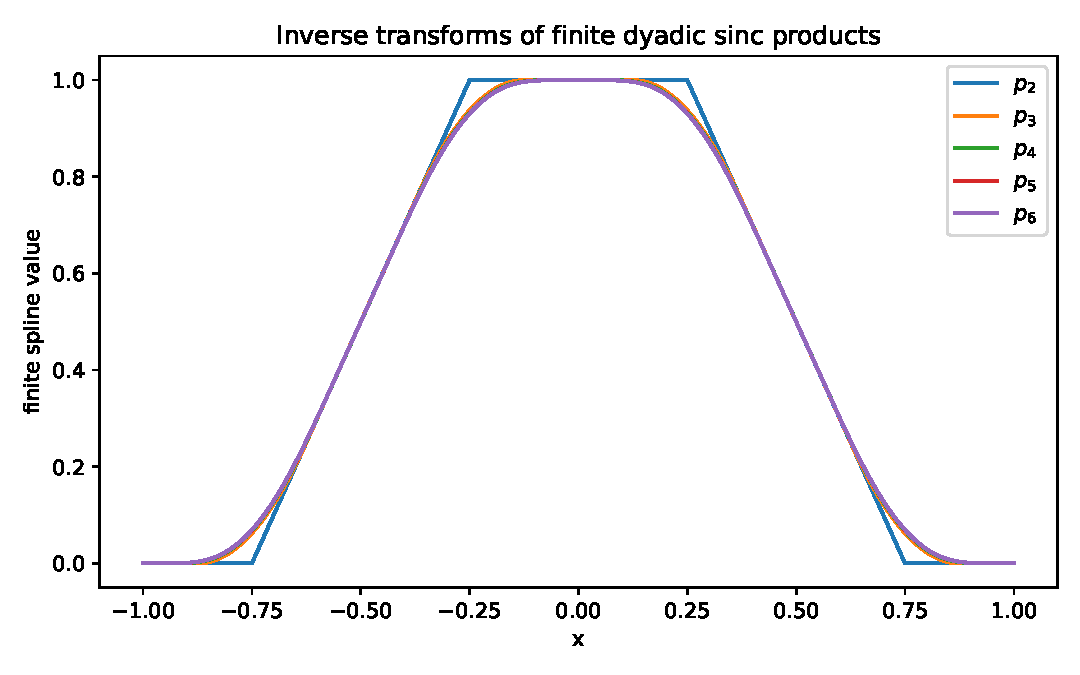
\includegraphics[width=0.88\textwidth]{finite_splines.pdf}
 \caption{The first several finite inverse transforms $p_N$.  Each new sinc
 factor convolves the preceding spline with a narrower centered box.}
 \label{fig:finite-splines}
\end{figure}

\subsection{Exact truncated-power representation}

Write
\begin{equation}
 \TM_k:=(-1)^{\pop(k)},
 \label{eq:thue-morse-sign}
\end{equation}
where $\pop(k)$ is the number of $1$'s in the binary expansion of $k$.
The following formula makes the spline structure and exact rational arithmetic
explicit.

\begin{theorem}[Finite spline with Thue--Morse knots]
For every $N\ge1$,
\begin{equation}
 \boxed{\displaystyle
 p_N(x)=\frac{2^{N(N-1)/2}}{(N-1)!}
 \sum_{k=0}^{2^N-1}\TM_k
 \left(x+A_N-\frac{k}{2^{N-1}}\right)_+^{N-1}.}
 \label{eq:truncated-power}
\end{equation}
The knots are
\begin{equation}
 t_{N,k}=-A_N+\frac{k}{2^{N-1}},
 \qquad 0\le k<2^N,
 \label{eq:knots}
\end{equation}
and consecutive knots are separated by $2^{1-N}$.
\end{theorem}

\begin{proof}
In the sense of distributions,
\[
 Db_k=2^k\left(\delta_{-2^{-k-1}}-\delta_{2^{-k-1}}\right).
\]
Differentiating the convolution \eqref{eq:prefix-convolution} once in every
factor gives
\[
 D^Np_N=(Db_0)*(Db_1)*\cdots*(Db_{N-1}).
\]
Choose a binary vector $(\beta_0,\ldots,\beta_{N-1})\in\{0,1\}^N$, where
$\beta_j=0$ selects the negative endpoint and $\beta_j=1$ the positive endpoint.
Starting from the all-negative position $-A_N$, changing the $j$-th choice adds
$2^{-j}$.  Hence the resulting atom is at
\[
 -A_N+\sum_{j=0}^{N-1}\beta_j2^{-j}
 =-A_N+\frac{k}{2^{N-1}},
 \qquad
 k=\sum_{j=0}^{N-1}\beta_j2^{N-1-j}.
\]
The sign is $(-1)^{\sum\beta_j}=\TM_k$ because reversing binary digits does not
change their sum.  The common magnitude is
\[
 \prod_{j=0}^{N-1}2^j=2^{N(N-1)/2}.
\]
Thus
\[
 D^Np_N=2^{N(N-1)/2}
 \sum_{k=0}^{2^N-1}\TM_k\delta_{t_{N,k}}.
\]
Since
\[
 D^N\frac{(x-t)_+^{N-1}}{(N-1)!}=\delta_t,
\]
integrating $N$ times from $-\infty$ and using compact support yields
\eqref{eq:truncated-power}.
\end{proof}

\begin{corollary}[Scaled cell formula]
Put
\begin{equation}
 y=2^{N-1}(x+A_N).
 \label{eq:scaled-y}
\end{equation}
Inside the support and away from the harmless $N=1$ jump convention,
\begin{equation}
 p_N(x)=\frac{2^{-(N-1)(N-2)/2}}{(N-1)!}
 \sum_{0\le k\le\floor y}\TM_k(y-k)^{N-1}.
 \label{eq:scaled-cell-formula}
\end{equation}
In particular, $p_N(x)\in\Q$ whenever $x\in\Q$.
\end{corollary}

\begin{proof}
Factor $2^{-(N-1)}$ from every truncated power in
\eqref{eq:truncated-power}.  Rationality is immediate.
\end{proof}

\subsection{Why dyadic points become cell midpoints}

\begin{definition}[Dyadic depth]
For a dyadic rational $x$, define
\begin{equation}
 \depth(x):=\min\{s\ge0:2^sx\in\Z\}.
 \label{eq:dyadic-depth}
\end{equation}
Thus a nonintegral dyadic has a unique reduced form $x=a/2^s$ with $a$ odd and
$s=\depth(x)$.
\end{definition}

\begin{lemma}[Exact midpoint alignment]
Let $-1<x<1$ be dyadic of depth $s$.  For every $N\ge s+1$, the point $x$ is the
midpoint of a unique polynomial cell of $p_N$, and that cell is precisely
\begin{equation}
 [x-2^{-N},\,x+2^{-N}].
 \label{eq:aligned-cell}
\end{equation}
\end{lemma}

\begin{proof}
By \eqref{eq:knots}, the cell width is $2^{1-N}$ and its half-width is $2^{-N}$.
Its midpoints are
\[
 \frac{t_{N,k}+t_{N,k+1}}2
 =-1+\frac{k+1}{2^{N-1}}.
\]
Since $N-1\ge s$, the number
\[
 J=2^{N-1}(1+x)
\]
is an integer.  Because $-1<x<1$, one has $1\le J\le2^N-1$.  Taking $k=J-1$
gives the required midpoint.  The claimed endpoints follow from the half-width.
\end{proof}

This exact alignment is the first reason the eventual law is finite.  It is not
true at a generic irrational point: as $N$ changes, the omitted tail generally
straddles a knot instead of remaining inside one polynomial piece.

\section{Head--tail self-similarity}

\subsection{The omitted tail is a scaled copy of the whole function}

Set
\begin{equation}
 \delta_N:=2^{-N}.
 \label{eq:deltaN}
\end{equation}
Splitting the infinite product after the first $N$ factors gives
\begin{equation}
 \Phi(t)=\Phi_N(t)\Phi(\delta_Nt).
 \label{eq:head-tail-fourier}
\end{equation}
Define the scaled density
\begin{equation}
 \upf_\delta(y):=\delta^{-1}\upf(y/\delta).
 \label{eq:scaled-up}
\end{equation}
Its Fourier transform is $\Phi(\delta t)$, and it is supported on
$[-\delta,\delta]$.  Fourier inversion of \eqref{eq:head-tail-fourier} yields
\begin{equation}
 \boxed{\upf=p_N*\upf_{\delta_N}.}
 \label{eq:head-tail-convolution}
\end{equation}
Probabilistically, the omitted random sum is $\delta_N$ times an independent
copy of the full random sum.


\begin{proposition}[Basic analytic properties and strict positivity]
\label{prop:basic-up}
The function $\upf$ is an even, nonnegative $C^\infty$ probability density with
support $[-1,1]$.  Moreover,
\begin{equation}
 \upf(0)=1,\qquad \upf(\pm1)=0,\qquad \upf(x)>0\quad(-1<x<1),
 \label{eq:basic-up-values}
\end{equation}
and it satisfies
\begin{equation}
 \upf'(x)=2\bigl(\upf(2x+1)-\upf(2x-1)\bigr).
 \label{eq:basic-up-diffeq}
\end{equation}
\end{proposition}

\begin{proof}
The random series in \eqref{eq:finite-random-sum}, continued to infinity,
converges almost surely and takes values in $[-1,1]$.  Its law is even and is the
convolution of the first box $b_0$ with the law of the remaining tail, hence it
has a nonnegative density of total mass one and Fourier transform $\Phi$.
For every fixed $K$, the first $K$ sinc factors give
$|\Phi(t)|\le C_K(1+|t|)^{-K}$, while all remaining factors have modulus at most
one.  Fourier inversion therefore gives derivatives of every order, so the
density is $C^\infty$.

The tail after $b_0$ is supported on $[-1/2,1/2]$, where $b_0$ is identically
one; consequently $\upf(0)=1$.  Continuity and compact support give
$\upf(\pm1)=0$.  Each finite convolution $p_N$ is strictly positive in the
interior of its support: if two nonnegative densities are positive on the
interiors of intervals, then their convolution is positive on the interior of
the sum interval because the overlap of the two positivity intervals has
positive length.  Now fix $|x|<1$ and choose $N$ so large that
$2\delta_N<1-|x|$.  For every $|y|\le\delta_N$,
\[
 |x-y|<1-\delta_N=A_N,
\]
so $p_N(x-y)>0$.  The head--tail convolution
\eqref{eq:head-tail-convolution} then implies $\upf(x)>0$.

Finally, splitting off the first box gives
$\upf=b_0*\upf_{1/2}$ and hence
\[
 \upf(x)=\int_{x-1/2}^{x+1/2}2\upf(2y)\,\dd y
        =\int_{2x-1}^{2x+1}\upf(z)\,\dd z.
\]
Differentiation proves \eqref{eq:basic-up-diffeq}.
\end{proof}

\subsection{The reciprocal sinc coefficients}

Near the origin define rational coefficients $a_m$ by
\begin{equation}
 \frac1{\Phi(z)}
 =\exp\!\left(\sum_{j=1}^{\infty}\alpha_j(2\pi z)^{2j}\right)
 =\sum_{m=0}^{\infty}a_m(2\pi z)^{2m}.
 \label{eq:reciprocal-series}
\end{equation}
The logarithmic expansion of $w/\sin w$ gives
\begin{equation}
 \alpha_j=\frac{\abs{B_{2j}}}
 {2j(2j)!\left(1-2^{-2j}\right)},
 \label{eq:alpha}
\end{equation}
where $B_{2j}$ are Bernoulli numbers.  Consequently
\begin{equation}
 a_0=1,
 \qquad
 ma_m=\sum_{j=1}^{m}j\alpha_j a_{m-j}.
 \label{eq:a-recurrence}
\end{equation}
Equivalently, with $Y_m$ denoting the complete exponential Bell polynomial,
\begin{equation}
 a_m=\frac1{m!}Y_m(1!\alpha_1,2!\alpha_2,\ldots,m!\alpha_m).
 \label{eq:a-Bell}
\end{equation}
The first values are
\begin{equation}
 \begin{aligned}
 a_0&=1,&
 a_1&=\frac1{18},&
 a_2&=\frac{31}{16200},\\
 a_3&=\frac{2347}{42865200},&
 a_4&=\frac{1904369}{1311675120000},&
 a_5&=\frac{3309760579}{88561680752160000}.
 \end{aligned}
 \label{eq:first-a}
\end{equation}
Every $\alpha_j$ is positive, so \eqref{eq:a-recurrence} also shows $a_m>0$.

\begin{proof}[Derivation of \eqref{eq:alpha}]
The standard Bernoulli expansion is
\[
 \log\frac{w}{\sin w}
 =\sum_{j=1}^{\infty}
 \frac{2^{2j-1}\abs{B_{2j}}}{j(2j)!}w^{2j}.
\]
Apply this to $w=\pi z/2^k$ and sum over $k\ge0$.  The geometric sum contributes
$(1-2^{-2j})^{-1}$.  Replacing $(\pi z)^{2j}$ by
$2^{-2j}(2\pi z)^{2j}$ gives \eqref{eq:alpha}.  Differentiating the formal
identity in \eqref{eq:reciprocal-series} with respect to
$X=(2\pi z)^2$ and comparing coefficients yields \eqref{eq:a-recurrence}; the
Bell-polynomial form is the exponential formula.
\end{proof}

\section{Exact polynomial deconvolution on one cell}

The usual Fourier argument gives an asymptotic differential expansion of $p_N$
in powers of $\delta_N^2$.  At an aligned dyadic point we can do better because
we are deconvolving a genuine polynomial on the whole support of the tail.

\subsection{A finite-dimensional operator identity}

Let
\begin{equation}
 M(z):=\int_{-1}^{1}\upf(y)e^{zy}\dd y.
 \label{eq:moment-generating}
\end{equation}
By the Fourier convention,
\begin{equation}
 M(z)=\Phi\!\left(\frac{iz}{2\pi}\right),
 \qquad
 \frac1{M(z)}=\sum_{m=0}^{\infty}(-1)^ma_mz^{2m}.
 \label{eq:M-reciprocal}
\end{equation}

\begin{lemma}[Exact inverse on polynomials]
Let $P$ be a polynomial of degree at most $D$, let $\delta>0$, and define
\begin{equation}
 (T_\delta P)(x):=\int_{-1}^{1}\upf(y)P(x-\delta y)\dd y.
 \label{eq:Tdelta}
\end{equation}
Then
\begin{equation}
 \boxed{\displaystyle
 P(x)=\sum_{m=0}^{\floor{D/2}}(-1)^ma_m\delta^{2m}
 (T_\delta P)^{(2m)}(x).}
 \label{eq:polynomial-inverse}
\end{equation}
The identity is algebraic and exact; no limiting argument and no analytic
convergence of the infinite reciprocal series are needed.
\end{lemma}

\begin{proof}
Let $D_x$ denote differentiation with respect to $x$.  Taylor's formula is finite
on polynomials, so
\[
 P(x-\delta y)=e^{-\delta yD_x}P(x)
\]
can be interpreted as a finite sum.  Integrating gives
\[
 T_\delta=M(-\delta D_x)=M(\delta D_x),
\]
because $\upf$ and hence $M$ are even.  On the vector space of polynomials of
degree at most $D$, the operator $D_x$ is nilpotent.  Therefore the formal
identity
\[
 M(z)^{-1}=\sum_{m\ge0}(-1)^ma_mz^{2m}
\]
may be substituted at $z=\delta D_x$ and truncates automatically after
$m=\floor{D/2}$.  This gives
\[
 T_\delta^{-1}=\sum_{m=0}^{\floor{D/2}}
 (-1)^ma_m\delta^{2m}D_x^{2m},
\]
which is \eqref{eq:polynomial-inverse}.
\end{proof}

\subsection{Locality converts the inverse into an identity for \texorpdfstring{$p_N$}{pN}}

\begin{lemma}[The tail sees only one polynomial piece]
Suppose $x$ is the midpoint of a cell of $p_N$, and let $P$ be the polynomial of
degree at most $N-1$ that agrees with $p_N$ on that cell.  Then, for every
$r\ge0$,
\begin{equation}
 (P*\upf_{\delta_N})^{(r)}(x)=\upf^{(r)}(x).
 \label{eq:local-jets}
\end{equation}
\end{lemma}

\begin{proof}
The cell is $[x-\delta_N,x+\delta_N]$, while
$\supp\upf_{\delta_N}=[-\delta_N,\delta_N]$.  Differentiating the smooth compactly
supported kernel in the convolution gives
\[
 \upf^{(r)}(x)
 =\int_{\R}p_N(z)\upf_{\delta_N}^{(r)}(x-z)\dd z.
\]
Only $z\in[x-\delta_N,x+\delta_N]$ contributes, and there $p_N(z)=P(z)$.
Replacing $p_N$ by $P$ therefore leaves the integral unchanged, proving
\eqref{eq:local-jets}.
\end{proof}

\begin{theorem}[Exact local differential formula]
If $x$ is the midpoint of a cell of $p_N$, then
\begin{equation}
 \boxed{\displaystyle
 p_N(x)=\sum_{m=0}^{\floor{(N-1)/2}}
 (-1)^ma_m4^{-mN}\upf^{(2m)}(x).}
 \label{eq:exact-local-expansion}
\end{equation}
More generally, for every $r\le N-1$,
\begin{equation}
 p_N^{(r)}(x)=
 \sum_{m=0}^{\floor{(N-1-r)/2}}
 (-1)^ma_m4^{-mN}\upf^{(r+2m)}(x).
 \label{eq:exact-local-derivative-expansion}
\end{equation}
\end{theorem}

\begin{proof}
With $P$ as in the preceding lemma, scaling in \eqref{eq:Tdelta} shows
$T_{\delta_N}P=P*\upf_{\delta_N}$.  Apply
\eqref{eq:polynomial-inverse} with $D=N-1$, evaluate at $x$, and use
\eqref{eq:local-jets}.  Since $\delta_N^{2m}=4^{-mN}$, this gives
\eqref{eq:exact-local-expansion}.  Differentiate the polynomial operator identity
$r$ times, or apply it to $P^{(r)}$, to obtain
\eqref{eq:exact-local-derivative-expansion}.
\end{proof}

\begin{remark}
For general $x$, the analogous formula is an all-orders asymptotic expansion.
At a cell midpoint it is exact because the nonlocal Fourier multiplier has been
reduced to a finite-dimensional polynomial operator.  This is the decisive
upgrade from asymptotic cancellation to exact extraction.
\end{remark}

\section{Dyadic derivative tiling and termination}

\subsection{The exact derivative-cell formula}

The Rvachev functional-differential equation is
\begin{equation}
 \upf'(x)=2\bigl(\upf(2x+1)-\upf(2x-1)\bigr).
 \label{eq:rvachev-equation}
\end{equation}
Iterating it produces a global Thue--Morse sum.

\begin{lemma}[Iterated derivative sum]
For every $r\ge0$ and $x\in\R$,
\begin{equation}
 \upf^{(r)}(x)=2^{\binom{r+1}{2}}
 \sum_{k=0}^{2^r-1}\TM_k\,
 \upf\!\left(2^r(x+1)-(2k+1)\right).
 \label{eq:global-derivative-sum}
\end{equation}
\end{lemma}

\begin{proof}
For $r=0$ the sum has one term and is $\upf(x)$.  Assume the formula at order
$r$.  Differentiate; the chain rule contributes $2^r$, and then apply
\eqref{eq:rvachev-equation} to every summand.  The positive branch has new index
$2k$ and sign $\TM_{2k}=\TM_k$; the negative branch has new index $2k+1$ and sign
$\TM_{2k+1}=-\TM_k$.  The factor gains $2^{r+1}$, changing
$2^{\binom{r+1}{2}}$ to $2^{\binom{r+2}{2}}$.  This is the formula at order
$r+1$.
\end{proof}

For $0\le k<2^r$ and $-1\le y\le1$, define the cell coordinate
\begin{equation}
 c_{r,k}(y):=-1+\frac{2k+1+y}{2^r}.
 \label{eq:cell-coordinate}
\end{equation}

\begin{theorem}[Exact derivative tiling]
For every $r\ge0$, $0\le k<2^r$, and $-1\le y\le1$,
\begin{equation}
 \boxed{\displaystyle
 \upf^{(r)}\bigl(c_{r,k}(y)\bigr)
 =2^{\binom{r+1}{2}}\TM_k\upf(y).}
 \label{eq:derivative-tiling}
\end{equation}
In particular,
\begin{equation}
 \upf^{(r)}\!\left(-1+\frac{2k+1}{2^r}\right)
 =2^{\binom{r+1}{2}}\TM_k.
 \label{eq:derivative-midpoint}
\end{equation}
\end{theorem}

\begin{proof}
Insert $x=c_{r,k}(y)$ into \eqref{eq:global-derivative-sum}.  The argument in the
$j$-th summand becomes
\[
 2^r(c_{r,k}(y)+1)-(2j+1)=2(k-j)+y.
\]
Because $\upf$ is supported on $[-1,1]$, only $j=k$ can contribute.  At
$y=\pm1$ a neighboring argument can also lie at an endpoint, but
$\upf(\pm1)=0$, so the same conclusion remains valid.  This proves
\eqref{eq:derivative-tiling}.  Set $y=0$ and use $\upf(0)=1$ for
\eqref{eq:derivative-midpoint}.
\end{proof}

\subsection{The dyadic jet stops at the dyadic depth}

\begin{theorem}[Dyadic derivative cutoff]
Let $-1<x<1$ be dyadic of depth $s\ge1$.  Then
\begin{align}
 \upf^{(r)}(x)&\ne0 &&(0\le r\le s),
 \label{eq:nonzero-low-derivatives}\\
 \upf^{(r)}(x)&=0 &&(r>s).
 \label{eq:zero-high-derivatives}
\end{align}
At the top nonzero order,
\begin{equation}
 \upf^{(s)}(x)=2^{\binom{s+1}{2}}\TM_k,
 \qquad
 k=\frac{2^s(1+x)-1}{2}.
 \label{eq:top-dyadic-derivative}
\end{equation}
\end{theorem}

\begin{proof}
Write $x=a/2^s$ in lowest terms, so $a$ is odd.  At $r=s$,
\[
 2^s(1+x)=2^s+a
\]
is odd.  Hence it is $2k+1$ for an integer $k$, and $x=c_{s,k}(0)$.
Equation \eqref{eq:derivative-midpoint} proves
\eqref{eq:top-dyadic-derivative}.

If $r>s$, then $2^r(1+x)=2^{r-s}(2^s+a)$ is an even integer, say $2h$.
Thus $x$ is a boundary of two order-$r$ derivative cells:
\[
 x=c_{r,h-1}(1)=c_{r,h}(-1).
\]
Applying \eqref{eq:derivative-tiling} and $\upf(\pm1)=0$ gives
\eqref{eq:zero-high-derivatives}.

Finally, if $r<s$, the number $2^r(1+x)$ is not an integer.  It belongs to the
interior of one order-$r$ cell, so $x=c_{r,k}(y)$ with $-1<y<1$.  The function
$\upf$ is strictly positive on $(-1,1)$; hence
\eqref{eq:derivative-tiling} is nonzero.  The case $r=0$ is the same positivity
statement.
\end{proof}

The function is $C^\infty$, yet its full derivative jet at a dyadic point is
finite: it ends exactly at the denominator depth.  This exceptional flatness is
the second reason the prefix expansion terminates.

\section{The eventual geometric law}

We now combine midpoint alignment, exact local deconvolution, and the derivative
cutoff.

\begin{theorem}[Exact eventual polynomialization]
\label{thm:eventual-law}
Let $x\in[-1,1]$ be dyadic, let
\begin{equation}
 s=\depth(x),\qquad d=\floor{s/2},\qquad \rho=\frac14,
 \label{eq:s-d-rho}
\end{equation}
and define $Q_n(x)=p_{n+1}(x)$.  There exist constants
$C_1(x),\ldots,C_d(x)$ such that
\begin{equation}
 \boxed{\displaystyle
 Q_n(x)=\upf(x)+\sum_{m=1}^{d}C_m(x)\rho^{mn}
 \qquad(n\ge s).}
 \label{eq:eventual-geometric-law}
\end{equation}
They are explicitly
\begin{equation}
 \boxed{\displaystyle
 C_m(x)=(-1)^ma_m\rho^m\upf^{(2m)}(x)
       =(-1)^ma_m4^{-m}\upf^{(2m)}(x).}
 \label{eq:Cm-derivative}
\end{equation}
For $-1<x<1$ and $s\ge2$, all $d$ correction coefficients are nonzero, so the
polynomial
\begin{equation}
 P_x(z):=\upf(x)+\sum_{m=1}^{d}C_m(x)z^m
 \label{eq:Px}
\end{equation}
has degree exactly $d$ and
\begin{equation}
 Q_n(x)=P_x(4^{-n})\qquad(n\ge s).
 \label{eq:polynomialized-sequence}
\end{equation}
\end{theorem}

\begin{proof}
First suppose $-1<x<1$ and $s\ge1$.  For $n\ge s$, put $N=n+1$.  Then
$N\ge s+1$, so $x$ is a cell midpoint of $p_N$ by the midpoint-alignment lemma.
The exact local formula \eqref{eq:exact-local-expansion} gives
\[
 Q_n(x)=p_{n+1}(x)
 =\sum_{m=0}^{\floor{n/2}}(-1)^ma_m4^{-m(n+1)}\upf^{(2m)}(x).
\]
Because $n\ge s$, every even order $2m\le s$ occurs in the displayed sum.
Every term with $2m>s$ vanishes by
\eqref{eq:zero-high-derivatives}.  Hence the surviving indices are exactly
$0\le m\le\floor{s/2}=d$, and
\[
 Q_n(x)=\upf(x)+\sum_{m=1}^{d}
 \left((-1)^ma_m4^{-m}\upf^{(2m)}(x)\right)4^{-mn}.
\]
This proves \eqref{eq:eventual-geometric-law} and
\eqref{eq:Cm-derivative}.

If $s\ge2$, then $2m\le s$ for $1\le m\le d$.  The derivative cutoff theorem
says these even derivatives are nonzero, and $a_m>0$, so every $C_m(x)$ is
nonzero.

It remains to cover depth $s=0$.  The possible points in $[-1,1]$ are
$-1,0,1$.  Every finite spline vanishes at $\pm1$ because its support is
$[-A_N,A_N]$ with $A_N<1$, while $\upf(\pm1)=0$.  At the origin, write
$p_N=b_0*(b_1*\cdots*b_{N-1})$.  The second factor is a probability density
supported in $[-1/2+2^{-N},1/2-2^{-N}]$, where the translate seen by $b_0$ has
constant value $1$; hence $p_N(0)=1=\upf(0)$.  Thus the formula holds with
$d=0$.
\end{proof}

\begin{corollary}[Number and ratios of the geometric corrections]
At a reduced dyadic point of depth $s$, at most the first $s$ user-indexed values
$Q_0,\ldots,Q_{s-1}$ are exceptional.  Thereafter there are
$d=\floor{s/2}$ correction modes.  The $m$-th mode has common ratio
\begin{equation}
 \frac{C_m4^{-m(n+1)}}{C_m4^{-mn}}=4^{-m}.
 \label{eq:mode-ratio}
\end{equation}
Thus each individual correction decreases geometrically in absolute value,
although cancellation between modes need not make the total error monotone.
\end{corollary}

\subsection{A cell formula for the correction coefficients}

For $1\le m\le d$, set $r=2m$ and define
\begin{equation}
 k_m=\floor{2^{2m-1}(1+x)},
 \qquad
 y_m=2^{2m}(1+x)-(2k_m+1).
 \label{eq:km-ym}
\end{equation}
Then $-1<y_m<1$; for $2m<s$ it lies
strictly in $(-1,1)$, and for $2m=s$ it is $0$.  From the derivative tiling,
\begin{equation}
 \upf^{(2m)}(x)=2^{m(2m+1)}\TM_{k_m}\upf(y_m).
 \label{eq:even-derivative-cell}
\end{equation}
Substitution into \eqref{eq:Cm-derivative} gives
\begin{equation}
 \boxed{\displaystyle
 C_m(x)=(-1)^ma_m2^{2m^2-m}\TM_{k_m}\upf(y_m).}
 \label{eq:Cm-cell}
\end{equation}
This expresses every geometric coefficient in terms of a lower-scale dyadic
value of the same function.  Rationality will also follow directly from the
extraction theorem below, so \eqref{eq:Cm-cell} then shows that all $C_m(x)$ are
rational.

\subsection{Derivative versions}

The same argument applies to derivatives of the finite splines.

\begin{corollary}[Eventual law for derivative approximants]
Let $0\le r\le s$, and evaluate the cellwise derivative of $p_{n+1}$ at $x$.
For every $n\ge s$,
\begin{equation}
 p_{n+1}^{(r)}(x)=\upf^{(r)}(x)
 +\sum_{m=1}^{\floor{(s-r)/2}}
 (-1)^ma_m4^{-m}\upf^{(r+2m)}(x)\,4^{-mn}.
 \label{eq:derivative-eventual-law}
\end{equation}
Hence the same $q$-extraction formula recovers $\upf^{(r)}(x)$, with
$d$ replaced by $\floor{(s-r)/2}$.
\end{corollary}

\begin{proof}
Use \eqref{eq:exact-local-derivative-expansion} and terminate it with
\eqref{eq:zero-high-derivatives}.
\end{proof}

\section{Exact extraction by a \texorpdfstring{$q$}{q}-Pochhammer filter}

\subsection{Shift-operator proof}

Let $E$ be the forward shift on sequences:
\begin{equation}
 (Ef)_n=f_{n+1}.
 \label{eq:shift}
\end{equation}
The constant sequence is an eigenvector of $E$ with eigenvalue $1$, and the
mode $\rho^{mn}$ is an eigenvector with eigenvalue $\rho^m$.  Therefore the
polynomial
\begin{equation}
 \mathcal P_d(E):=\prod_{m=1}^{d}(E-\rho^m)
 \label{eq:filter-polynomial}
\end{equation}
annihilates every correction mode in \eqref{eq:eventual-geometric-law}.  On the
constant term it acts by
\begin{equation}
 \mathcal P_d(1)=\prod_{m=1}^{d}(1-\rho^m)=(\rho;\rho)_d.
 \label{eq:filter-at-one}
\end{equation}
Here
\begin{equation}
 (a;q)_d:=\prod_{r=0}^{d-1}(1-aq^r),
 \qquad
 (q;q)_d=\prod_{r=1}^{d}(1-q^r)
 \label{eq:q-pochhammer}
\end{equation}
is the finite $q$-Pochhammer symbol.

The finite $q$-binomial theorem gives
\begin{equation}
 \prod_{m=1}^{d}(z-\rho^m)
 =\sum_{j=0}^{d}(-1)^{d-j}
 \rho^{\binom{d-j+1}{2}}
 \qbinom{d}{j}{\rho}\,z^j,
 \label{eq:q-binomial-polynomial}
\end{equation}
where
\begin{equation}
 \qbinom{d}{j}{q}:=\frac{(q;q)_d}{(q;q)_j(q;q)_{d-j}}
 \label{eq:gaussian-binomial}
\end{equation}
is the Gaussian binomial coefficient.

\begin{theorem}[Single-formula exact extractor]
\label{thm:exact-extractor}
Under the hypotheses of \cref{thm:eventual-law}, let $n_0\ge s$.  Then
\begin{equation}
 \boxed{\displaystyle
 \upf(x)=\frac1{(\rho;\rho)_d}
 \sum_{j=0}^{d}(-1)^{d-j}\rho^{\binom{d-j+1}{2}}
 \qbinom{d}{j}{\rho}\,Q_{n_0+j}(x),
 \qquad \rho=\frac14.}
 \label{eq:extractor-rho}
\end{equation}
Equivalently,
\begin{equation}
 \boxed{\displaystyle
 \upf(x)=\sum_{j=0}^{d}
 \frac{(-1)^{d-j}\rho^{\binom{d-j+1}{2}}}
 {(\rho;\rho)_j(\rho;\rho)_{d-j}}\,Q_{n_0+j}(x).}
 \label{eq:extractor-pochhammer}
\end{equation}
\end{theorem}

\begin{proof}
Apply \eqref{eq:filter-polynomial} to
\eqref{eq:eventual-geometric-law} at index $n_0$.  Every mode with
$1\le m\le d$ is killed by its factor $E-\rho^m$, while the constant survives
with multiplier $(\rho;\rho)_d$.  Hence
\[
 \mathcal P_d(E)Q_{n_0}=(\rho;\rho)_d\upf(x).
\]
Expand $\mathcal P_d$ by \eqref{eq:q-binomial-polynomial} and divide by
$(\rho;\rho)_d$ to get \eqref{eq:extractor-rho}.  Substitute
\eqref{eq:gaussian-binomial} for \eqref{eq:extractor-pochhammer}.
\end{proof}

\begin{corollary}[One completely explicit finite formula]
\label{cor:fully-explicit}
Let $N_j=n_0+j+1$ and $A_{N_j}=1-2^{-N_j}$.  Substitution of the exact spline
formula into \eqref{eq:extractor-pochhammer} gives
\begin{equation}
\boxed{\begin{aligned}
 \upf(x)=\sum_{j=0}^{d}&
 \frac{(-1)^{d-j}\rho^{\binom{d-j+1}{2}}}
 {(\rho;\rho)_j(\rho;\rho)_{d-j}}
 \frac{2^{N_j(N_j-1)/2}}{(N_j-1)!}\\[-0.1em]
 &\times\sum_{k=0}^{2^{N_j}-1}\TM_k
 \left(x+1-2^{-N_j}-\frac{k}{2^{N_j-1}}\right)_+^{N_j-1},
 \qquad \rho=\frac14.
\end{aligned}}
\label{eq:fully-explicit}
\end{equation}
Every sum and product in \eqref{eq:fully-explicit} is finite.  Taking $n_0=s$
gives the smallest guaranteed formula, involving exactly $d+1$ finite splines.
\end{corollary}

\begin{proof}
Use $Q_{n_0+j}=p_{N_j}$ in \eqref{eq:extractor-pochhammer} and substitute
\eqref{eq:truncated-power}.  No passage to a limit remains.
\end{proof}

\subsection{Integer-coefficient base-4 form}

The inversion identity
\begin{equation}
 \qbinom{d}{j}{q^{-1}}=q^{-j(d-j)}\qbinom{d}{j}{q}
 \label{eq:q-inversion}
\end{equation}
and
\begin{equation}
 (1/4;1/4)_d
 =4^{-d(d+1)/2}\prod_{r=1}^{d}(4^r-1)
 \label{eq:pochhammer-base4}
\end{equation}
convert \eqref{eq:extractor-rho} to an especially useful rational formula.

\begin{corollary}[Common-denominator integer formula]
For every $n_0\ge s$,
\begin{equation}
 \boxed{\displaystyle
 \upf(x)=
 \frac{\displaystyle\sum_{j=0}^{d}(-1)^{d-j}
 4^{\binom{j+1}{2}}\qbinom{d}{j}{4}\,Q_{n_0+j}(x)}
 {\displaystyle\prod_{r=1}^{d}(4^r-1)}.}
 \label{eq:extractor-base4}
\end{equation}
All coefficients in the numerator are integers and the common denominator is
odd.
\end{corollary}

\begin{proof}
Insert \eqref{eq:q-inversion} with $q=4$ and
\eqref{eq:pochhammer-base4} into \eqref{eq:extractor-rho}.  The total power of
$4$ multiplying the $j$-th term is
\[
 \binom{d+1}{2}-\binom{d-j+1}{2}-j(d-j)
 =\binom{j+1}{2}.
\]
Gaussian binomial coefficients at the integer base $4$ are integers.
\end{proof}

\begin{corollary}[Rationality at dyadic points]
For every dyadic $x\in[-1,1]$, one has $\upf(x)\in\Q$.
\end{corollary}

\begin{proof}
Every finite value $Q_{n_0+j}(x)$ is rational by the truncated-power formula,
and every extraction weight is rational.  Equation
\eqref{eq:extractor-pochhammer} finishes the proof.
\end{proof}

This gives a direct proof of classical dyadic rationality from finite
Fourier-product splines.

\subsection{First weight vectors}

Writing
\begin{equation}
 \upf(x)=\sum_{j=0}^{d}W_{d,j}Q_{n_0+j}(x),
 \label{eq:weight-definition}
\end{equation}
the first vectors are
\begin{align}
 d=0:&\quad (1),\label{eq:w0}\\
 d=1:&\quad \left(-\frac13,\frac43\right),\label{eq:w1}\\
 d=2:&\quad \left(\frac1{45},-\frac49,\frac{64}{45}\right),\label{eq:w2}\\
 d=3:&\quad \left(-\frac1{2835},\frac4{135},-\frac{64}{135},
                    \frac{4096}{2835}\right),\label{eq:w3}\\
 d=4:&\quad \left(\frac1{722925},-\frac4{8505},\frac{64}{2025},
       -\frac{4096}{8505},\frac{1048576}{722925}\right).
 \label{eq:w4}
\end{align}
The weights depend only on the denominator depth through $d$, not on the
numerator of $x$ and not on the chosen valid starting index $n_0$.

\subsection{Stability of the signed formula}

Alternating extrapolation weights can sometimes be numerically dangerous.  Here
the total variation is uniformly small.

\begin{proposition}[Uniform weight bound]
For $0<\rho<1$,
\begin{equation}
 \sum_{j=0}^{d}\abs{W_{d,j}}
 =\frac{(-\rho;\rho)_d}{(\rho;\rho)_d}.
 \label{eq:weight-variation}
\end{equation}
At $\rho=1/4$,
\begin{equation}
 \sum_{j=0}^{d}\abs{W_{d,j}}
 <\frac{(-1/4;1/4)_\infty}{(1/4;1/4)_\infty}
 =1.969260353668269\ldots.
 \label{eq:weight-bound-numeric}
\end{equation}
Consequently, if each input value has absolute error at most $\eta$, the
extracted value has error less than $1.97\eta$.
\end{proposition}

\begin{proof}
Use \eqref{eq:extractor-rho}, discard the alternating signs, and replace
$j$ by $d-r$:
\[
 \sum_{j=0}^{d}\abs{W_{d,j}}
 =\frac1{(\rho;\rho)_d}
 \sum_{r=0}^{d}\rho^{r(r+1)/2}\qbinom{d}{r}{\rho}.
\]
The finite $q$-binomial theorem with positive signs says that the numerator is
\[
 \prod_{m=1}^{d}(1+\rho^m)=(-\rho;\rho)_d.
\]
The finite products increase to the displayed infinite-product ratio.  The
error statement is the triangle inequality.
\end{proof}

\section{The Vandermonde system and recovery of every coefficient}

The extraction formula gives the constant without solving a system explicitly.
The full geometric law is recovered from exactly the same data.

\subsection{Polynomial interpolation on geometric nodes}

Fix a valid starting index $n_0\ge s$ and define
\begin{equation}
 A_m:=C_m(x)\rho^{mn_0},
 \qquad
 R(z):=\upf(x)+\sum_{m=1}^{d}A_mz^m.
 \label{eq:R-polynomial}
\end{equation}
Then
\begin{equation}
 R(\rho^j)=Q_{n_0+j}(x),
 \qquad 0\le j\le d.
 \label{eq:R-samples}
\end{equation}
Therefore the unknown vector $(\upf(x),A_1,\ldots,A_d)^T$ is the solution of
\begin{equation}
 \begin{pmatrix}
 1&1&1&\cdots&1\\
 1&\rho&\rho^2&\cdots&\rho^d\\
 1&\rho^2&\rho^4&\cdots&\rho^{2d}\\
 \vdots&\vdots&\vdots&&\vdots\\
 1&\rho^d&\rho^{2d}&\cdots&\rho^{d^2}
 \end{pmatrix}
 \begin{pmatrix}
 \upf(x)\\A_1\\A_2\\\vdots\\A_d
 \end{pmatrix}
 =
 \begin{pmatrix}
 Q_{n_0}(x)\\Q_{n_0+1}(x)\\Q_{n_0+2}(x)\\\vdots\\Q_{n_0+d}(x)
 \end{pmatrix}.
 \label{eq:vandermonde-system}
\end{equation}
The determinant is
\begin{equation}
 \prod_{0\le a<b\le d}(\rho^b-\rho^a)\ne0,
 \label{eq:vandermonde-det}
\end{equation}
so the solution is unique over $\Q$.

The Lagrange form is
\begin{equation}
 R(z)=\sum_{j=0}^{d}Q_{n_0+j}(x)\ell_j(z),
 \qquad
 \ell_j(z)=\prod_{\substack{0\le r\le d\\r\ne j}}
 \frac{z-\rho^r}{\rho^j-\rho^r}.
 \label{eq:lagrange-R}
\end{equation}
Thus every coefficient is available in one expression:
\begin{equation}
 \boxed{\displaystyle
 C_m(x)=\rho^{-mn_0}
 \sum_{j=0}^{d}Q_{n_0+j}(x)[z^m]\ell_j(z),
 \qquad 0\le m\le d,}
 \label{eq:all-coefficients}
\end{equation}
where $C_0(x)=\upf(x)$.  A convenient $q$-Pochhammer normalization of the
Lagrange denominator is
\begin{equation}
 \prod_{\substack{0\le r\le d\\r\ne j}}(\rho^j-\rho^r)
 =(-1)^j\rho^{j(j-1)/2+j(d-j)}
 (\rho;\rho)_j(\rho;\rho)_{d-j}.
 \label{eq:lagrange-denominator}
\end{equation}
Setting $z=0$ in \eqref{eq:lagrange-R} reduces exactly to
\eqref{eq:extractor-pochhammer}.

\subsection{Minimality}

\begin{proposition}[Why $d+1$ samples are generically necessary]
For an interior dyadic point of depth $s\ge2$, the $d+1$ sequences
\begin{equation}
 1,\rho^n,\rho^{2n},\ldots,\rho^{dn}
 \label{eq:basis-sequences}
\end{equation}
all occur with nonzero coefficients in \eqref{eq:eventual-geometric-law} and are
linearly independent.  Consequently, without additional derivative information,
$d+1$ scalar samples are the minimal generic amount of data needed to identify
all coefficients, including $\upf(x)$.
\end{proposition}

\begin{proof}
Nonvanishing was proved in \cref{thm:eventual-law}.  Linear independence follows
by evaluating a putative relation at $d+1$ consecutive integers; the resulting
coefficient matrix is the nonsingular Vandermonde matrix
\eqref{eq:vandermonde-system}.  Fewer than $d+1$ equations cannot uniquely
determine $d+1$ unconstrained coefficients.
\end{proof}

\section{Annihilating recurrences and onset diagnostics}

Because the eventual sequence is a finite sum of exponentials, it satisfies a
constant-coefficient recurrence.

\begin{theorem}[Exact eventual recurrence]
For every $n\ge s$,
\begin{equation}
 \boxed{\displaystyle
 \prod_{m=0}^{d}(E-\rho^m)Q_n(x)=0.}
 \label{eq:annihilator}
\end{equation}
Equivalently,
\begin{equation}
 \sum_{j=0}^{d+1}(-1)^{d+1-j}
 \rho^{\binom{d+1-j}{2}}
 \qbinom{d+1}{j}{\rho}\,Q_{n+j}(x)=0.
 \label{eq:expanded-recurrence}
\end{equation}
\end{theorem}

\begin{proof}
The factor $E-1$ kills the constant term, and $E-\rho^m$ kills the $m$-th
geometric mode.  The expanded form is the finite $q$-binomial theorem.
\end{proof}

This recurrence is useful in three ways.

\begin{enumerate}
\item It gives an exact check that a proposed starting index is late enough.
\item If a dyadic fraction has not first been reduced, the smallest recurrence
order detected from exact data reveals the effective value $d=\floor{s/2}$.
\item In floating-point calculations, its residual measures both evaluation
error and contamination by pre-asymptotic values.
\end{enumerate}

The recurrence order is $d+1$ because it includes the constant eigenvalue $1$.
The extraction filter in \cref{thm:exact-extractor} omits $E-1$, preserving the
constant while annihilating all error modes.

\section{Worked examples}

\subsection{Depth zero and one}

At $x=0$, every $Q_n(0)=1$, so no extrapolation is needed.  At $x=\pm1$, every
$Q_n(x)=0$.  For $x=\pm1/2$, the depth is $s=1$ and $d=0$, hence
\begin{equation}
 Q_n(\pm1/2)=\upf(\pm1/2)=\frac12\qquad(n\ge1).
 \label{eq:half-example}
\end{equation}
The possibly convention-dependent endpoint value of the first box $Q_0$ is one
of the allowed initial exceptions.

\subsection{One correction mode: \texorpdfstring{$x=3/4$}{x = 3/4}}

Here $s=2$, $d=1$, and the exact finite values are
\begin{equation}
 Q_2\!\left(\frac34\right)=\frac1{16},
 \qquad
 Q_3\!\left(\frac34\right)=\frac{13}{192}.
 \label{eq:three-quarter-data}
\end{equation}
The $d=1$ extractor is
\begin{equation}
 \upf(x)=\frac{4Q_{n_0+1}(x)-Q_{n_0}(x)}3.
 \label{eq:d1-extractor}
\end{equation}
At $n_0=2$ it gives
\begin{equation}
 \upf\!\left(\frac34\right)
 =\frac{4(13/192)-1/16}{3}=\frac5{72}.
 \label{eq:up-three-quarter}
\end{equation}
Moreover $3/4$ is the midpoint of the $k=3$ second-derivative cell, so
\begin{equation}
 \upf''\!\left(\frac34\right)=2^{\binom32}\TM_3\upf(0)=8.
 \label{eq:second-derivative-three-quarter}
\end{equation}
Since $a_1=1/18$,
\begin{equation}
 C_1=-\frac1{18}\frac14\cdot8=-\frac19.
\end{equation}
Therefore the complete tail is
\begin{equation}
 \boxed{\displaystyle
 Q_n\!\left(\frac34\right)=\frac5{72}-\frac19\,4^{-n}
 \qquad(n\ge2).}
 \label{eq:three-quarter-law}
\end{equation}
The threshold is sharp here: the displayed law does not hold at $n=1$.

\subsection{Odd depth: \texorpdfstring{$x=7/8$}{x = 7/8}}

For $x=7/8$, one has $s=3$ but still $d=1$.  Exact extraction gives
\begin{equation}
 \upf\!\left(\frac78\right)=\frac1{288},
 \qquad
 Q_n\!\left(\frac78\right)=\frac1{288}-\frac1{18}4^{-n}
 \quad(n\ge3).
 \label{eq:seven-eighths-law}
\end{equation}
The odd top derivative $\upf^{(3)}(7/8)$ is nonzero, but only even derivatives
enter the centered-tail deconvolution; hence the mode count remains
$\floor{3/2}=1$.

\subsection{Two correction modes: \texorpdfstring{$x=15/16$}{x = 15/16}}

Now $s=4$ and $d=2$.  The three required finite values are
\begin{equation}
 Q_4\!\left(\frac{15}{16}\right)=\frac1{24576},\qquad
 Q_5\!\left(\frac{15}{16}\right)=\frac{121}{1966080},\qquad
 Q_6\!\left(\frac{15}{16}\right)=\frac{6331}{94371840}.
 \label{eq:fifteen-sixteenths-data}
\end{equation}
Using \eqref{eq:w2},
\begin{align}
 \upf\!\left(\frac{15}{16}\right)
 &=\frac1{45}Q_4-\frac49Q_5+\frac{64}{45}Q_6\notag\\
 &=\boxed{\frac{143}{2073600}}.
 \label{eq:fifteen-sixteenths-value}
\end{align}
The coefficients can be read from derivatives.  At derivative order $2$,
$15/16$ maps to $y=3/4$ with positive Thue--Morse sign, so
\begin{equation}
 \upf''\!\left(\frac{15}{16}\right)
 =8\upf\!\left(\frac34\right)=\frac59.
 \label{eq:fifteen-second}
\end{equation}
At derivative order $4$, the point itself is a cell midpoint with positive sign,
so
\begin{equation}
 \upf^{(4)}\!\left(\frac{15}{16}\right)=2^{\binom52}=1024.
 \label{eq:fifteen-fourth}
\end{equation}
Consequently
\begin{align}
 C_1&=-\frac1{18}\frac14\frac59=-\frac5{648},\\
 C_2&=\frac{31}{16200}\frac1{16}\,1024=\frac{248}{2025}.
\end{align}
The full exact law is
\begin{equation}
 \boxed{\displaystyle
 Q_n\!\left(\frac{15}{16}\right)
 =\frac{143}{2073600}-\frac5{648}4^{-n}
 +\frac{248}{2025}4^{-2n},\qquad n\ge4.}
 \label{eq:fifteen-sixteenths-law}
\end{equation}
Cancelling only the first mode changes the observed decay from approximately
$4^{-n}$ to exactly a multiple of $16^{-n}$; cancelling both returns the limit
with zero residual in exact arithmetic.

\begin{figure}[htbp]
 \centering
 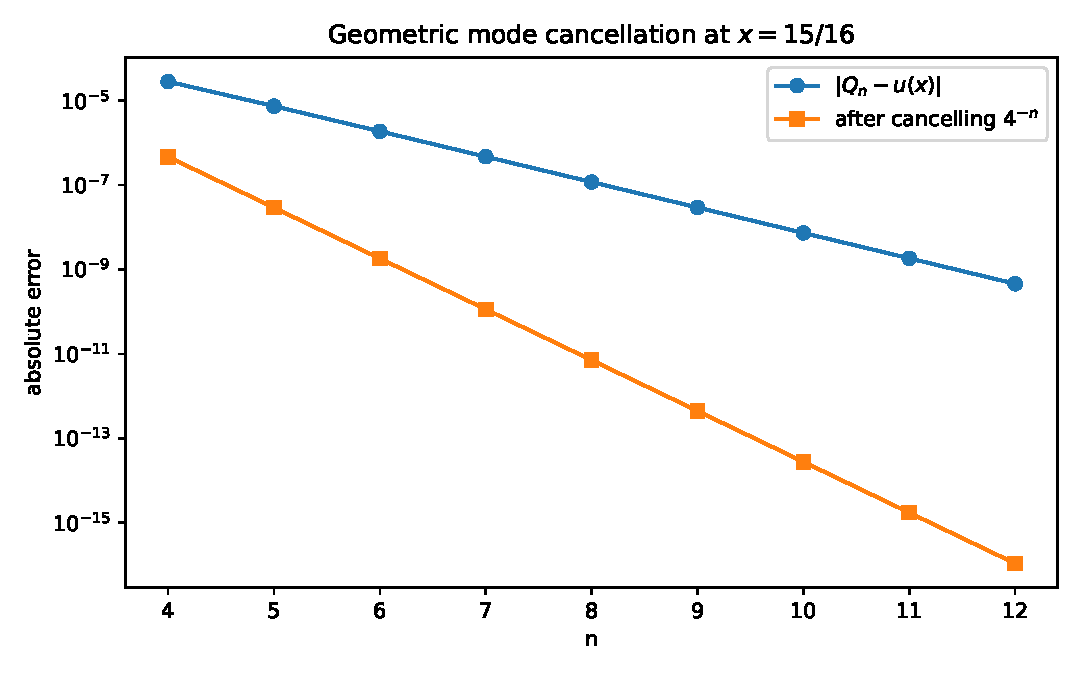
\includegraphics[width=0.88\textwidth]{geometric_mode_cancellation.pdf}
 \caption{At $x=15/16$, one $q$-Richardson step cancels the $4^{-n}$ mode and
 leaves only the $4^{-2n}=16^{-n}$ mode.  The two-mode formula cancels both
 exactly.}
 \label{fig:mode-cancellation}
\end{figure}

\subsection{A three-mode example}

For $x=63/64$, $s=6$ and $d=3$.  Solving the four-by-four rational system gives
\begin{equation}
 \begin{aligned}
 Q_n\!\left(\frac{63}{64}\right)
 ={}&\frac{1153}{561842749440}
 -\frac{143}{18662400}4^{-n}
 +\frac{31}{3645}4^{-2n}\\
 &\hspace{1.6cm}
 -\frac{4806656}{2679075}4^{-3n},\qquad n\ge6.
 \end{aligned}
 \label{eq:sixty-three-law}
\end{equation}
The exact value is obtained from $Q_6,Q_7,Q_8,Q_9$ with the $d=3$ vector
\eqref{eq:w3}.  Large-looking correction coefficients are harmless because they
multiply very small powers $4^{-mn}$.

\subsection{Symmetry}

Since every finite box is even, every $p_N$ and $\upf$ are even.  Therefore all
formulas at $x$ immediately give the corresponding formulas at $-x$:
\begin{equation}
 Q_n(-x)=Q_n(x),\qquad \upf(-x)=\upf(x),\qquad C_m(-x)=C_m(x).
 \label{eq:even-symmetry}
\end{equation}

\section{Exact extraction algorithm}

\begin{algorithm}[Dyadic rational extraction]
\label{alg:extraction}
Given a dyadic rational $x\in[-1,1]$:
\begin{enumerate}
\item Reduce $x$ and determine the smallest $s$ such that $2^sx\in\Z$.
\item Set $d=\floor{s/2}$ and choose any $n_0\ge s$; the smallest guaranteed
choice is $n_0=s$.
\item Compute the $d+1$ exact rational spline values
\[
 Q_{n_0}(x),Q_{n_0+1}(x),\ldots,Q_{n_0+d}(x)
\]
using \eqref{eq:truncated-power} or \eqref{eq:scaled-cell-formula}.
\item Compute the exact weights
\[
 W_{d,j}=\frac{(-1)^{d-j}\rho^{\binom{d-j+1}{2}}}
 {(\rho;\rho)_j(\rho;\rho)_{d-j}},\qquad \rho=\frac14.
\]
\item Return
\[
 \upf(x)=\sum_{j=0}^{d}W_{d,j}Q_{n_0+j}(x).
\]
\item Optionally solve \eqref{eq:vandermonde-system} to obtain every $C_m$, and
verify the next unused value with \eqref{eq:eventual-geometric-law} or the
recurrence \eqref{eq:expanded-recurrence}.
\end{enumerate}
\end{algorithm}

\subsection{Exact arithmetic at aligned points}

At a valid index $n\ge s$, let $N=n+1$ and use the scaled coordinate
$y=2^{N-1}(x+A_N)$.  Midpoint alignment makes $2y$ an odd integer.  Therefore
\eqref{eq:scaled-cell-formula} can be evaluated without any fractional power in
the summation:
\begin{equation}
 p_N(x)=\frac{1}{2^{N(N-1)/2}(N-1)!}
 \sum_{0\le k\le\floor y}\TM_k(2y-2k)^{N-1}.
 \label{eq:integer-midpoint-evaluation}
\end{equation}
This is the form used by the accompanying code.  It uses only integer powers,
integer Thue--Morse signs, and one final rational normalization.

\subsection{Pseudocode}

\begin{lstlisting}[style=code,language=Python,caption={Core exact extraction logic.}]
s = dyadic_depth(x)
d = s // 2
rho = Fraction(1, 4)

values = [up_prefix(x, s + j) for j in range(d + 1)]
weights = []
for j in range(d + 1):
    r = d - j
    weights.append(
        (-1)**r * rho**(r*(r+1)//2)
        / (qpoch(rho, j) * qpoch(rho, r))
    )

exact_up_x = sum(w*q for w, q in zip(weights, values))
\end{lstlisting}

The complete file \texttt{verify\_dyadic\_up\_extraction.py} includes exact
finite-spline evaluation, $q$-Pochhammer and Gaussian-binomial routines,
rational Gauss--Jordan elimination, analytic coefficient reconstruction from
derivative cells, recurrence checks, CSV generation, and figures.

\section{Computational verification}

All numerical claims in this section were obtained with
\texttt{fractions.Fraction}; no floating-point fitting was used.  The script
exhaustively tested every reduced dyadic point in $[-1,1]$ of depth at most seven.
There are
\begin{equation}
 3+\sum_{s=1}^{7}2^s=257
 \label{eq:point-count}
\end{equation}
such points when $-1,0,1$ are included at depth zero.

For each point the program performed the following independent exact checks:

\begin{enumerate}
\item extraction from four different valid starting windows returned the same
rational value;
\item the Vandermonde-fitted coefficients reproduced six consecutive finite
approximants beyond the onset;
\item the fitted coefficients agreed term by term with
$(-1)^ma_m4^{-m}\upf^{(2m)}(x)$, with derivatives evaluated by the exact cell
tiling;
\item the $q$-binomial annihilating recurrence had zero residual for six
consecutive indices.
\end{enumerate}

The run completed
\begin{equation}
 \begin{array}{lr}
 \text{sequence and window identities} & 2570,\\
 \text{analytic-versus-fitted coefficient entries} & 941,\\
 \text{annihilating recurrence identities} & 1542,
 \end{array}
 \label{eq:verification-counts}
\end{equation}
with every equality exact.  Representative values and the complete run summary
are stored in the companion CSV and text files included with the archive.

\begin{table}[htbp]
\centering
\small
\caption{Representative exact geometric laws $Q_n=L+\sum_{m=1}^dC_m4^{-mn}$.}
\label{tab:representative-laws}
\begin{tabularx}{\textwidth}{@{}c c c X@{}}
\toprule
$x$ & $s$ & $d$ & Exact law, valid for $n\ge s$\\
\midrule
$3/4$ & $2$ & $1$ & $\displaystyle Q_n=\frac5{72}-\frac19 4^{-n}$\\[0.4em]
$7/8$ & $3$ & $1$ & $\displaystyle Q_n=\frac1{288}-\frac1{18}4^{-n}$\\[0.4em]
$15/16$ & $4$ & $2$ & $\displaystyle Q_n=\frac{143}{2073600}-\frac5{648}4^{-n}+\frac{248}{2025}4^{-2n}$\\[0.4em]
$5/16$ & $4$ & $2$ & $\displaystyle Q_n=\frac{1767743}{2073600}+\frac{67}{648}4^{-n}+\frac{248}{2025}4^{-2n}$\\[0.4em]
$31/32$ & $5$ & $2$ & $\displaystyle Q_n=\frac{19}{33177600}-\frac1{2592}4^{-n}+\frac{124}{2025}4^{-2n}$\\
\bottomrule
\end{tabularx}
\end{table}

\section{Further consequences and extensions}

\subsection{Exact rather than asymptotic Richardson acceleration}

For an arbitrary point, the $M$-sample signed geometric Richardson combination
cancels the first $M-1$ terms of an asymptotic expansion and leaves a smaller
remainder.  At a dyadic point of depth $s$, choose $M=d+1$.  There is no
remainder: every possible even-derivative term after order $2d$ is exactly zero.
Thus the same filter changes status from an accelerator to a finite exact
reconstruction operator.

This also explains why using more than $d+1$ samples is unnecessary in exact
arithmetic.  Extra samples are useful only for consistency checking, for
averaging noisy approximate evaluations, or when the denominator depth is not
known reliably.

\subsection{A rational generating function for the eventual sequence}

Let $n\ge s$ and write $R_k=Q_{s+k}(x)$.  From
\eqref{eq:eventual-geometric-law},
\begin{equation}
 \sum_{k=0}^{\infty}R_kz^k
 =\frac{\upf(x)}{1-z}
 +\sum_{m=1}^{d}\frac{C_m(x)\rho^{ms}}{1-\rho^mz}.
 \label{eq:eventual-generating-function}
\end{equation}
Hence the tail generating function is rational, with denominator dividing
\begin{equation}
 (1-z)\prod_{m=1}^{d}(1-\rho^mz).
 \label{eq:generating-denominator}
\end{equation}
The recurrence \eqref{eq:annihilator} is the coefficient form of this rationality.

\subsection{Finite differences and mode peeling}

The first difference removes the constant:
\begin{equation}
 Q_{n+1}-Q_n
 =\sum_{m=1}^{d}C_m(\rho^m-1)\rho^{mn}.
 \label{eq:first-difference}
\end{equation}
Applying $E-\rho$ removes the slowest remaining mode; applying
$E-\rho^2$ next removes the second, and so on.  This gives a sequential
``mode-peeling'' interpretation of the product filter.  It is useful for
symbolic diagnostics and for displaying the progressively faster slopes in a
log-error plot.

\subsection{General geometric scales}

The polynomial-deconvolution lemma does not depend on the number $2$.  Suppose a
compactly supported smooth density $u$ admits a head--tail identity
\begin{equation}
 u=p_N*u_{\lambda^N}
 \label{eq:general-head-tail}
\end{equation}
with $0<\lambda<1$, and the relevant finite prefix is polynomial on a full tail
neighborhood of a point.  If the reciprocal Fourier symbol has only even powers,
then the correction modes are
\begin{equation}
 \lambda^{2mN}=(\lambda^2)^{mN}.
 \label{eq:general-modes}
\end{equation}
Whenever an independent structural theorem makes the derivative jet finite at
the point, the same argument produces an exact $q$-interpolation formula with
$q=\lambda^2$.  In the Rvachev case, $\lambda=1/2$ and therefore $q=1/4$.
The uniform dyadic knot alignment and the exact derivative cutoff are the
special features that make the theorem especially clean here.

\subsection{What changes away from dyadic points}

At a non-dyadic point, two obstructions appear.

\begin{enumerate}
\item The tail interval $[x-2^{-N},x+2^{-N}]$ generally crosses a knot of $p_N$,
so one polynomial no longer describes the entire convolution neighborhood.
\item The derivative jet $\upf^{(r)}(x)$ does not terminate at a finite order in
general.
\end{enumerate}

The all-orders expansion and $q$-Richardson acceleration remain useful, but the
finite exact formula should not be expected.  This contrast sharply identifies
the arithmetic-geometric role of dyadic points.

\section{Conclusions}

For a dyadic point $x=a/2^s$, the finite sinc-product splines contain the exact
value $\upf(x)$ in a surprisingly small amount of data.  After index $n=s$ the
entire sequence is a degree-$\floor{s/2}$ polynomial in $4^{-n}$.  The mechanism
is exact at every stage:

\begin{enumerate}
\item the finite Fourier product is a uniform-knot Thue--Morse spline;
\item the point becomes the midpoint of a cell once $n\ge s$ in the user
indexing;
\item the omitted tail is supported precisely inside that cell;
\item reciprocal-sinc deconvolution is finite on the cell polynomial;
\item the derivative tiling kills all orders above $s$;
\item a $q$-Pochhammer filter annihilates the remaining geometric modes.
\end{enumerate}

The final reconstruction is the single formula
\[
 \upf(x)=\sum_{j=0}^{d}
 \frac{(-1)^{d-j}4^{-\binom{d-j+1}{2}}}
 {(1/4;1/4)_j(1/4;1/4)_{d-j}}\,Q_{n_0+j}(x),
 \qquad d=\floor{s/2},\ n_0\ge s,
\]
or, equivalently, the integer-coefficient base-$4$ Gaussian-binomial formula
\eqref{eq:extractor-base4}.  The Vandermonde interpolation polynomial recovers
all correction coefficients as well.  In exact arithmetic this is a finite
algorithm for the rational dyadic values of Rvachev's up-function; in numerical
arithmetic it is also stable, with weight amplification uniformly below $1.97$.

\appendix

\section{Proof of the Lagrange weight formula}

For completeness, evaluate the Lagrange basis \eqref{eq:lagrange-R} at zero.
The numerator is
\begin{equation}
 \prod_{\substack{0\le r\le d\\r\ne j}}(-\rho^r)
 =(-1)^d\rho^{d(d+1)/2-j}.
 \label{eq:lagrange-zero-numerator}
\end{equation}
For $r<j$,
\[
 \rho^j-\rho^r=-\rho^r(1-\rho^{j-r}),
\]
so those factors contribute
\[
 (-1)^j\rho^{j(j-1)/2}(\rho;\rho)_j.
\]
For $r>j$,
\[
 \rho^j-\rho^r=\rho^j(1-\rho^{r-j}),
\]
so those factors contribute
\[
 \rho^{j(d-j)}(\rho;\rho)_{d-j}.
\]
Their quotient is
\begin{align}
 \ell_j(0)
 &=\frac{(-1)^{d-j}
 \rho^{d(d+1)/2-j-j(j-1)/2-j(d-j)}}
 {(\rho;\rho)_j(\rho;\rho)_{d-j}}\notag\\
 &=\frac{(-1)^{d-j}\rho^{(d-j)(d-j+1)/2}}
 {(\rho;\rho)_j(\rho;\rho)_{d-j}},
 \label{eq:lagrange-weight-derived}
\end{align}
which is exactly \eqref{eq:extractor-pochhammer}.

\section{Finite \texorpdfstring{$q$}{q}-binomial identities used in the article}

The finite $q$-binomial theorem is
\begin{equation}
 (a;q)_d=\sum_{r=0}^{d}(-1)^rq^{\binom r2}
 \qbinom{d}{r}{q}a^r.
 \label{eq:finite-q-binomial}
\end{equation}
With $a=q/z$, multiplication by $z^d$ yields
\begin{align}
 \prod_{m=1}^{d}(z-q^m)
 &=z^d(q/z;q)_d\notag\\
 &=\sum_{r=0}^{d}(-1)^rq^{r(r+1)/2}
   \qbinom{d}{r}{q}z^{d-r}.
 \label{eq:q-product-expanded-r}
\end{align}
Putting $j=d-r$ gives \eqref{eq:q-binomial-polynomial}.  Replacing $a$ by
$-q$ in \eqref{eq:finite-q-binomial} gives
\begin{equation}
 \prod_{m=1}^{d}(1+q^m)
 =\sum_{r=0}^{d}q^{r(r+1)/2}\qbinom{d}{r}{q},
 \label{eq:q-positive-sum}
\end{equation}
which proves the variation formula \eqref{eq:weight-variation}.

\section{Reproducibility files}

The archive accompanying this article contains:

\begin{description}[leftmargin=3.8cm,style=nextline]
\item[\texttt{dyadic\_up\_extraction.tex}]
The complete LaTeX source.
\item[\texttt{dyadic\_up\_extraction.pdf}]
The rendered article.
\item[\texttt{verify\_dyadic\_up\_extraction.py}]
A documented exact-arithmetic implementation and verification suite.
\item[\texttt{sample\_sequences.csv}]
Representative finite values, exact limits, and errors.
\item[\texttt{geometric\_coefficients.csv}]
Fitted exact coefficients for representative points.
\item[\texttt{verification\_report.txt}]
The exhaustive depth-seven verification summary and initial coefficient tables.
\item[\texttt{finite\_splines.pdf/.png}]
The generated finite-spline figure.
\item[\texttt{geometric\_mode\_cancellation.pdf/.png}]
The generated mode-cancellation figure.
\end{description}

To reproduce the tables and figures, run
\begin{lstlisting}[style=code,language=bash]
python verify_dyadic_up_extraction.py --out-dir . --max-depth 7
\end{lstlisting}
The exact verification can be run without plotting dependencies by adding
\texttt{--skip-plots}.

\begin{thebibliography}{99}

\bibitem{proveit-primary}
V.~Reshetnikov,
\emph{The Fabius Function and Rvachev's Up-Function: Exact arithmetic,
probability, Fourier analysis, and corrected sharp asymptotics},
\texttt{ProveIt} repository documentation,
\url{https://github.com/VladimirReshetnikov/ProveIt/tree/main/Analysis/FabiusFunction/docs/Fabius_Function_and_Rvachev_Up}.

\bibitem{proveit-frontier}
V.~Reshetnikov,
\emph{Exponents and $q$-Series Frontiers}, especially the finite sinc-product
spline, head--tail, all-orders, and signed geometric Richardson sections,
\texttt{ProveIt} repository documentation,
\url{https://github.com/VladimirReshetnikov/ProveIt/tree/main/Analysis/FabiusFunction/docs/semi-formalized-research-frontiers/drafts/exponents-and-q-series}.

\bibitem{arias1982}
J.~Arias de Reyna,
\emph{An infinitely differentiable function with compact support: Definition and
properties}, English translation of the 1982 paper,
\href{https://arxiv.org/abs/1702.05442}{arXiv:1702.05442} (2017).

\bibitem{arias-arithmetic}
J.~Arias de Reyna,
\emph{Arithmetic of the Fabius function},
\href{https://arxiv.org/abs/1702.06487}{arXiv:1702.06487} (2017).

\bibitem{dlmf-q}
NIST Digital Library of Mathematical Functions,
\emph{Chapter 17: $q$-Hypergeometric and Related Functions}, especially
Section 17.2,
\url{https://dlmf.nist.gov/17.2}.

\bibitem{gasper-rahman}
G.~Gasper and M.~Rahman,
\emph{Basic Hypergeometric Series}, 2nd ed.,
Encyclopedia of Mathematics and its Applications 96,
Cambridge University Press, 2004.

\end{thebibliography}

\end{document}
